\entry{Semana del 02/06/2025}
Ya están completamente diseñadas las placas, tanto con las borneras de 2 pines a PCB, de ELEMON, como con los jacks BNC-PCB de 90° de iUrbaNet. 

\section{PCB con Borneras.}
\begin{figure}[!ht]
	\begin{minipage}[c]{0.3325\textwidth}
			\begin{subfigure}{\textwidth}
					\centering
					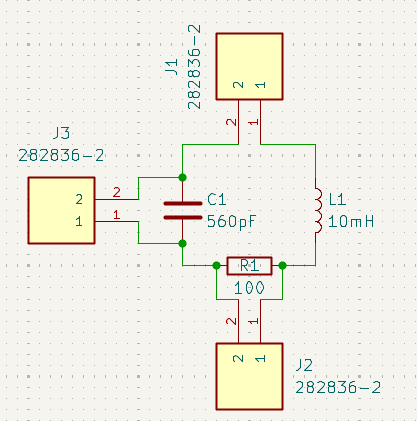
\includegraphics[width=0.978\textwidth]{Figures/02_06_2025/Schematic_borneras}
					\captionsetup{width=0.8\textwidth}
					\subcaption{}
				\end{subfigure}
		\end{minipage}\begin{minipage}[c]{0.332149\textwidth}
			\begin{subfigure}{\textwidth}
					\centering
					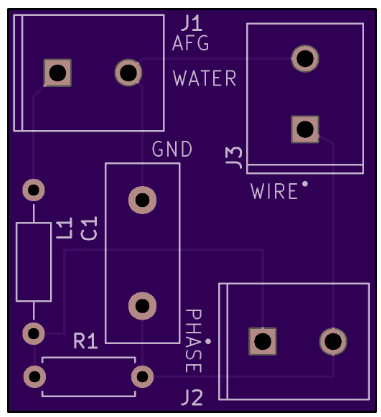
\includegraphics[width=0.978\textwidth]{Figures/02_06_2025/PCB_Top_borneras.png}
					\captionsetup{width=0.8\textwidth}
					\subcaption{}
				\end{subfigure}
		\end{minipage}\begin{minipage}[c]{0.3321249\textwidth}
		\begin{subfigure}{\textwidth}
			\centering
			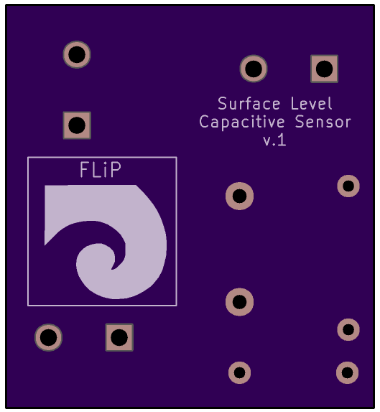
\includegraphics[width=0.978\textwidth]{Figures/02_06_2025/PCB_Bottom_borneras}
			\captionsetup{width=0.8\textwidth}
			\subcaption{}
		\end{subfigure}
	\end{minipage}
	\caption{A la izquierda el esquema del circuito eléctrico que corresponde a la placa. A la derecha la vista superior e inferior de la placa terminada.} %  y  
	\label{fig:}
\end{figure}




\begin{figure}[!ht]
	\begin{minipage}[c]{0.5\textwidth}
			\begin{subfigure}{\textwidth}
					\centering
					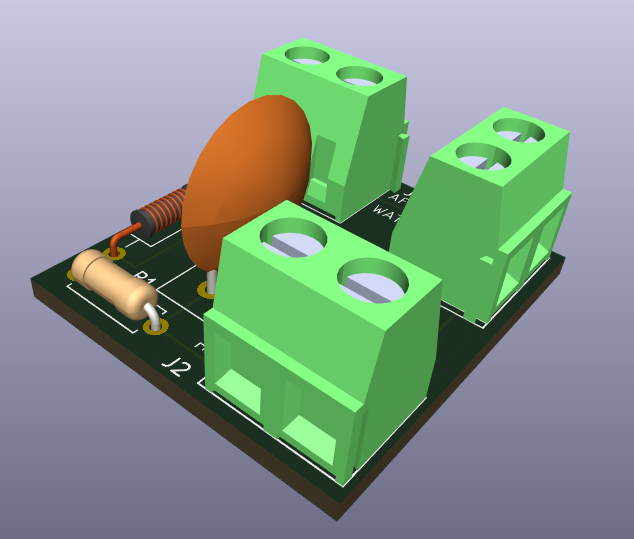
\includegraphics[width=0.82\textwidth]{Figures/02_06_2025/PCB_3D_perfil_borneras1}
					\captionsetup{width=0.8\textwidth}
					\subcaption{}
				\end{subfigure}
		\end{minipage}\begin{minipage}[c]{0.49\textwidth}
			\begin{subfigure}{\textwidth}
					\centering
					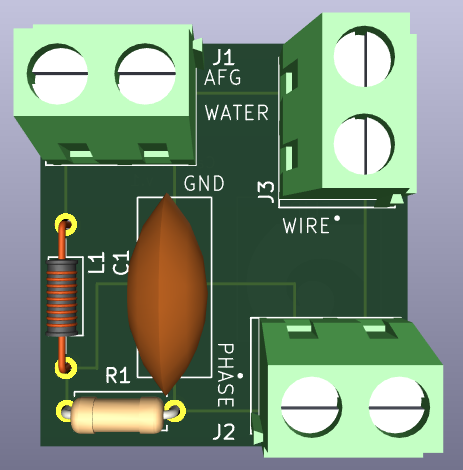
\includegraphics[width=0.78\textwidth]{Figures/02_06_2025/PCB_3D_top_borneras}
					\captionsetup{width=0.8\textwidth}
					\subcaption{}
				\end{subfigure}
		\end{minipage}
	\caption{Dos vistas del Modelo 3D de la placa con sus componentes.}
	\label{fig:}
\end{figure}

La placa terminada tiene dimensiones 26.0 x 28.5mm. El costo estimado de 3 placas debería ser USD 5.70 según OSHPARK. % $ $ 

% 5 Figures/02_06_2025/PCB_Bottom_borneras
% Figures/02_06_2025/PCB_Top_BNC

\section{PCB con BNC.}
\begin{figure}[!ht]
	\begin{minipage}[c]{0.3325\textwidth}
		\begin{subfigure}{\textwidth}
			\centering
			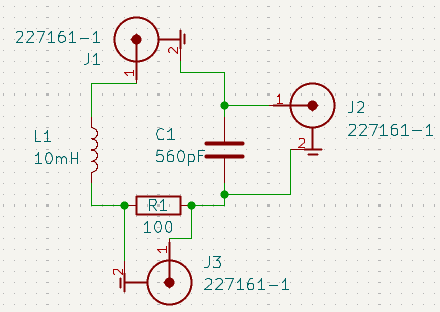
\includegraphics[width=0.978\textwidth]{Figures/02_06_2025/Schematic_BNC}
			\captionsetup{width=0.8\textwidth}
			\subcaption{}
		\end{subfigure}
	\end{minipage}\begin{minipage}[c]{0.332149\textwidth}
		\begin{subfigure}{\textwidth}
			\centering
			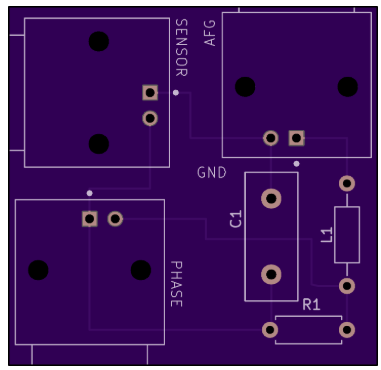
\includegraphics[width=0.978\textwidth]{Figures/02_06_2025/PCB_Top_BNC.png}
			\captionsetup{width=0.78\textwidth}
			\subcaption{}
		\end{subfigure}
	\end{minipage}\begin{minipage}[c]{0.3321249\textwidth}
		\begin{subfigure}{\textwidth}
			\centering
			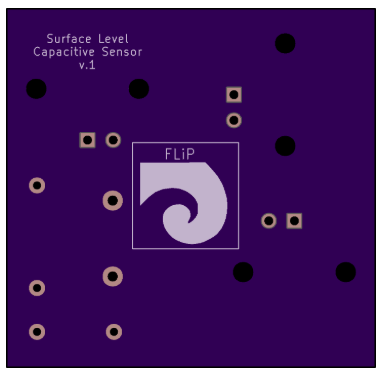
\includegraphics[width=0.978\textwidth]{Figures/02_06_2025/PCB_Bottom_BNC}
			\captionsetup{width=0.8\textwidth}
			\subcaption{}
		\end{subfigure}
	\end{minipage}
	\caption{A la izquierda el esquema del circuito eléctrico que corresponde a la placa. A la derecha la vista superior e inferior de la placa terminada.}
	\label{fig:}
\end{figure}





\begin{figure}[!ht]
	\begin{minipage}[c]{0.5\textwidth}
		\begin{subfigure}{\textwidth}
			\centering
			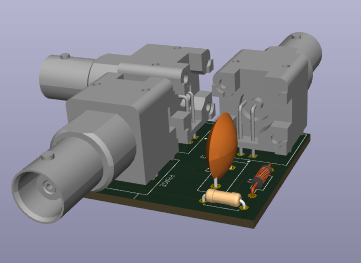
\includegraphics[width=0.98\textwidth]{Figures/02_06_2025/PCB_3D_perfil_BNC}
			\captionsetup{width=0.8\textwidth}
			\subcaption{}
		\end{subfigure}
	\end{minipage}\begin{minipage}[c]{0.49\textwidth}
		\begin{subfigure}{\textwidth}
			\centering
			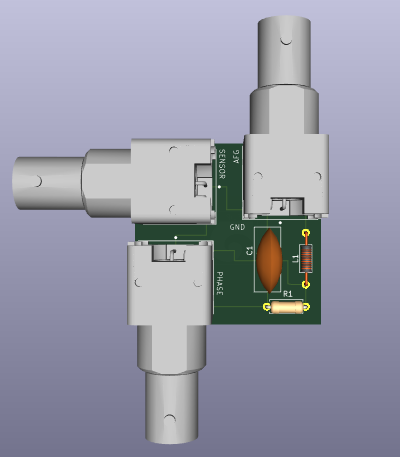
\includegraphics[width=0.8\textwidth,angle=90,origin=c]{Figures/02_06_2025/PCB_3D_top_BNC}
			\captionsetup{width=0.8\textwidth}
			\subcaption{}
		\end{subfigure}
	\end{minipage}
	\caption{Dos vistas del Modelo 3D de la placa con sus componentes.}
	\label{fig:}
\end{figure}



Las dimensiones de la placa son 36.5 x 35.5mm. El costo de 3 placas debería ser USD 10.05 según OSHPARK. % $ $

\section{Componentes.}
Los componentes para las placas son las resistencias, capacitancias e inductancias que ya tenemos en el Laboratorio, los agujeros se eligieron según el pin pitch y dimensiones de estos. Después para las conexiones al exterior se utilizarían:

\begin{itemize}
	\item Bornera de 2 pines: TE Connectivity 282836-2 de ELEMON.
	\item Jack BNC-PCB 90°: de iUrbaNet, el modelo que declaran no lo encontré, así que usé las plantillas del de TE Connectivity 227161-1.
\end{itemize}

\section{Miércoles 04/06/2025.} % {}
No llegó el adaptador AC/DC para la placa de adquisición. Fuimos a preguntar arriba a los Labos y a Compu para pedir uno prestado pero no tenían tampoco, ni el jack para soldarlo a un cable y usar una fuente DC regulable de los Labos.

\section{Viernes 06/06/2025.}
Pablo consiguió la fuente así que podemos empezar a usar la placa. Esta placa (modelo PS 3001) requiere sí o sí potencia externa ya que los 5V a 0.5A máx del USB no le da para operar.  

IMPORTANTE: Conectar primero la potencia externa para que luego al conectar el USB pida los requerimientos mínimos de potencia a la computadora.

\begin{figure}[!ht]
	\begin{minipage}[c]{0.5\textwidth}
			\begin{subfigure}{\textwidth}
					\centering
					\includegraphics[width=0.8\textwidth]{"Figures/09_06_2025/Esquema placa"}
					\captionsetup{width=0.8\textwidth}
					\subcaption{}
				\end{subfigure}
		\end{minipage}\begin{minipage}[c]{0.49\textwidth}
			\begin{subfigure}{\textwidth}
					\centering
					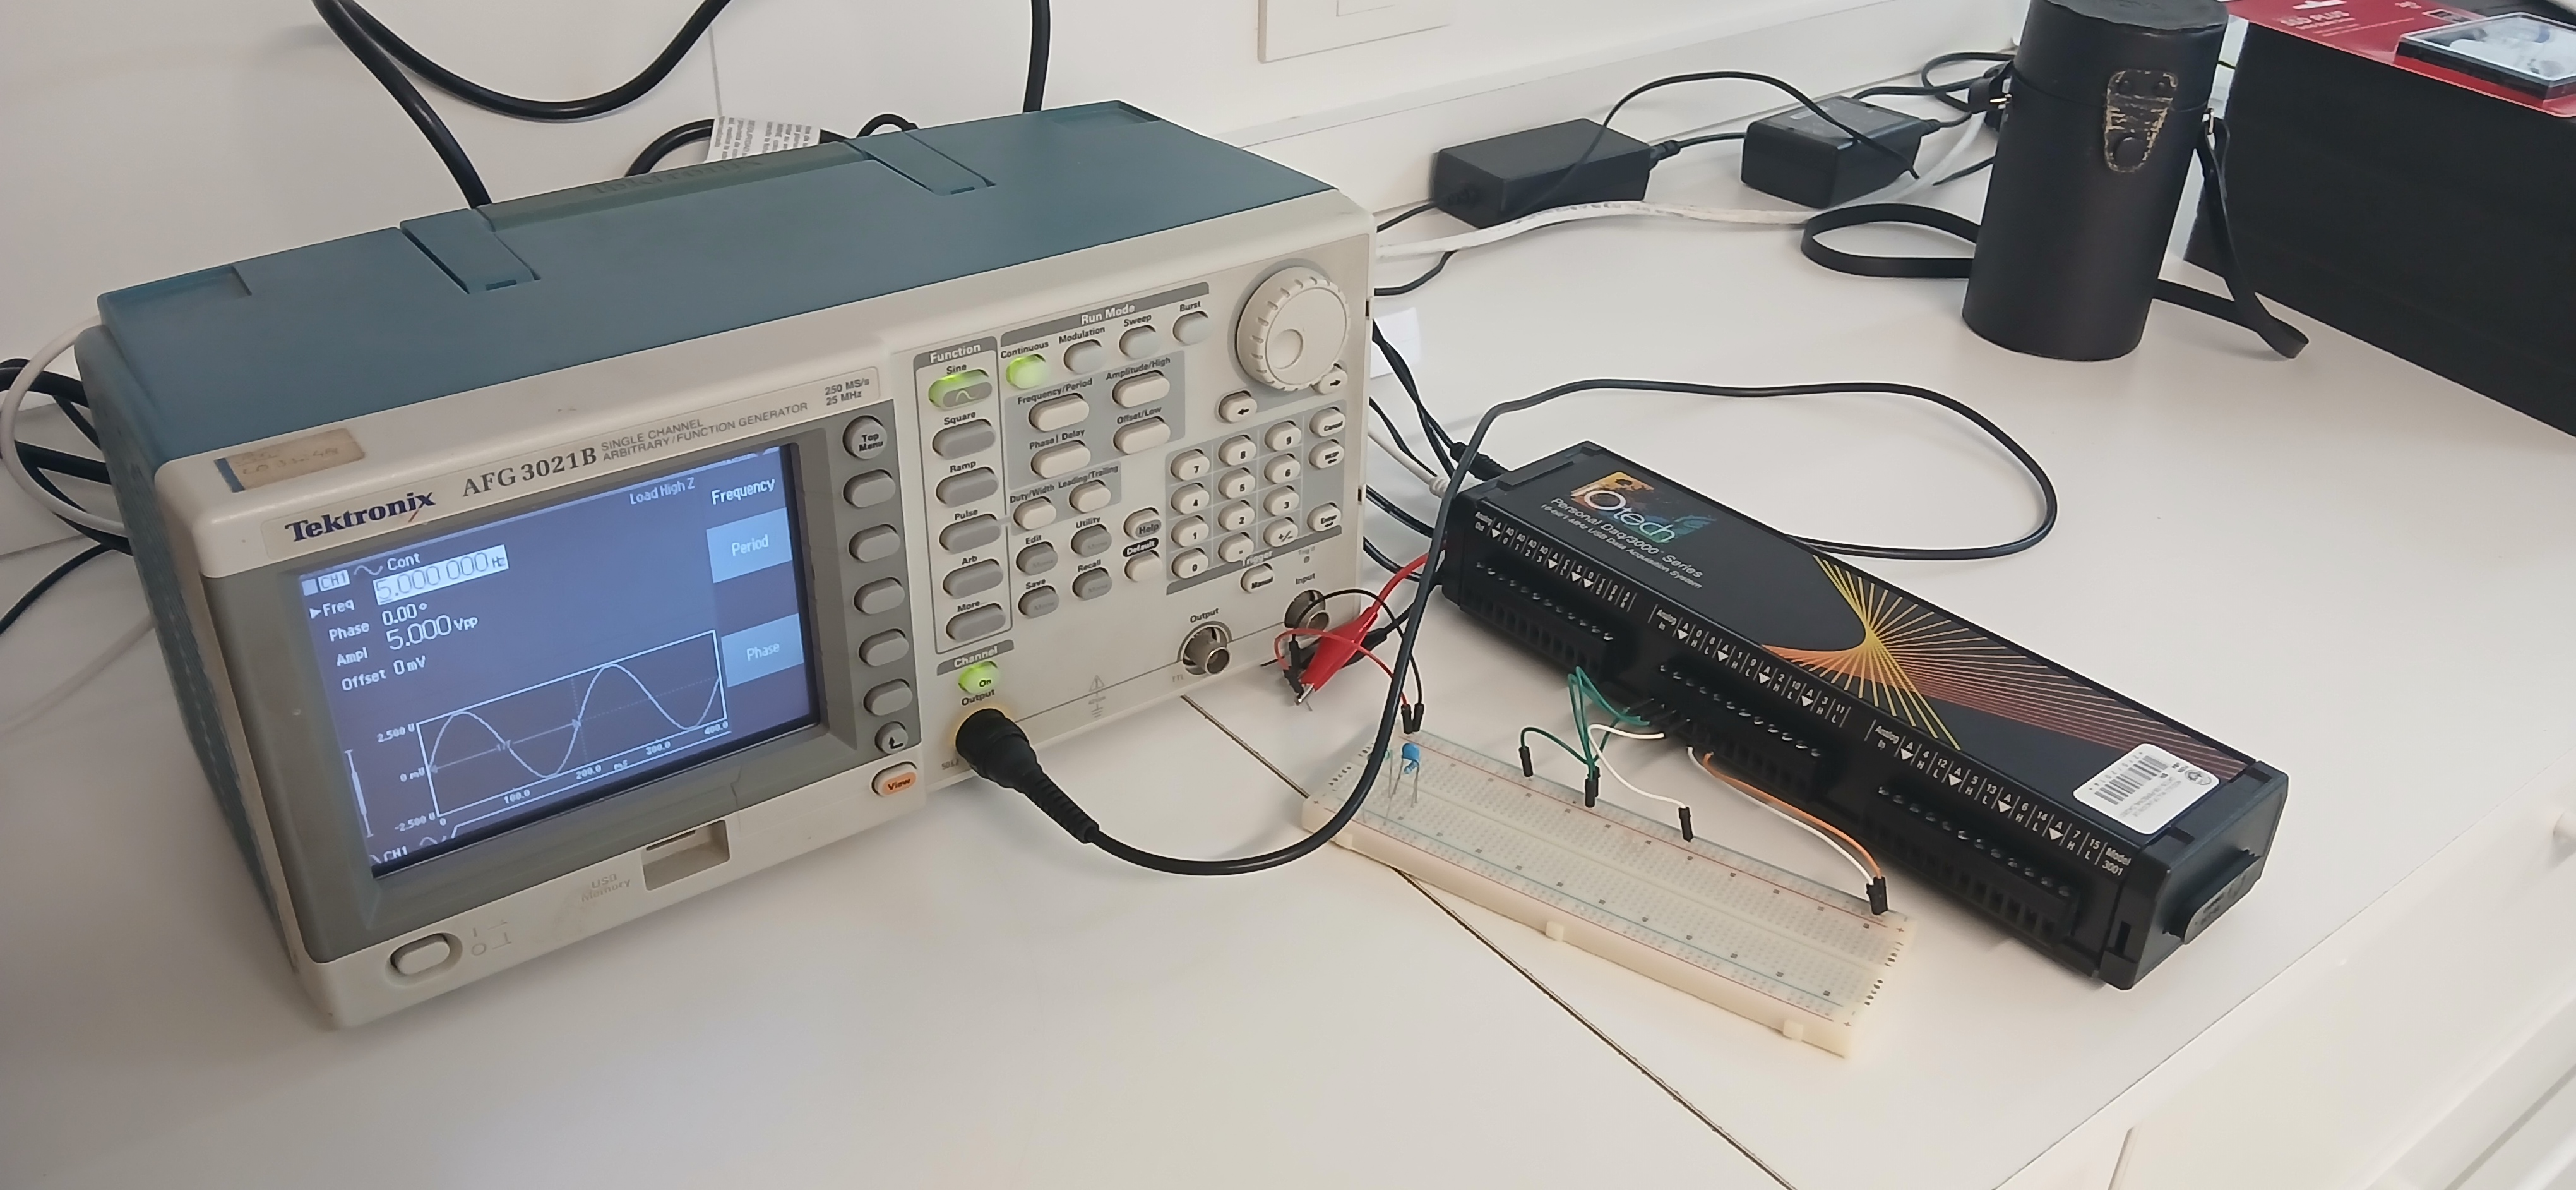
\includegraphics[width=0.8\textwidth]{Figures/02_06_2025/Foto placa.jpg}
					\captionsetup{width=0.8\textwidth}
					\subcaption{}
				\end{subfigure}
		\end{minipage}
	\caption{Esquema de la placa y una foto de la misma conectada.}
	\label{fig:placa_esquema_y_foto}
\end{figure}



DaqView en Windows 10 no estuvo funcionando, tira algunos errores de cosas no declaradas que no pude arreglar. Intenté también ejecutarlo en modo compatibilidad con Windows XP y 7 pero daba los mismos errores. Principalmente que cuando está activa, si bien parece leer correctamente los valores de los distintos canales, no podía guardar estos valores en disco. Sin embargo sirvió para bajar los drivers de la placa y el .dll necesario para la API. 
DaqView no funcionó pero pyIOTech, un wrapper de la API en C en Python, con los drivers de la placa sí.

El procedimiento para descargar todo en Windows 10 sería:
\begin{itemize}
	\item Descargar DaqView para los drivers desde la páina de Digilent. 
	\item Ejecutar la intalación.
	\item Clonar el repositorio de Github de PYIOTech: "https://github.com/fake-name/PyIOTech".
	\item Seguir las instrucciones de instalación, corriendo el "python setup.py install" desde el directorio donde se clonó el repositorio.
	\item Buscar la ubicación del paquete instalado, en mi caso: ``C:/Users/Marcelo/AppData/Local/Programs/
	
	Python/Python310/Lib/site-packages/PyIOTech". % " 
	\item Abrir daq.py y cambiar la ubicación del .dll según donde se haya instalado DaqView. En mi caso: ``C:/Program Files (x86)/DaqX/Drivers/USB\_x64". % " 
	\item Cambiar entonces la línea "dll = find\_library('daqx')" por "dll = r``C:/Program Files (x86)/DaqX/
	
	Drivers/USB\_x64/DaqX64.dll"". IMPORTANTE: Asegurarse de usar el .dll de 64 bits porque el de 32 bits tira error (no es compatible con Python de 64 bits). % " 
	\item En DaqView agregar la placa para que instale los dirvers correspondientes.
	\item Correr para encontrar el nombre de tu placa:
	\begin{lstlisting} 
		from PyIOTech import daq
		
		count = daq.GetDeviceCount()  
		print("Dispositivos encontrados:", count)
		name = daq.GetDeviceList()
	\end{lstlisting}
	En mi caso b'PersonalDaq3001{374679}'.
\end{itemize} % # daq 

Después de esto no quedó mucho tiempo pero seguí el ejemplo de PyIOTech para tomar una medición puntual del canal 0 configurado en diferencial. 

\begin{lstlisting}
from PyIOTech import daq, daqh
	
device_name = b'PersonalDaq3001{374679}' 
channel = 0
gain = daqh.DgainX1
flags = daqh.DafAnalog | daqh.DafUnsigned | daqh.DafBipolar | daqh.DafDifferential
max_voltage = 10.0
bit_depth = 16
	
dev = daq.daqDevice(device_name)
data = dev.AdcRd(channel, gain, flags)
data = data*max_voltage*2/(2**bit_depth) - max_voltage
dev.Close()
\end{lstlisting}

Un par de cosas sobre el funcionamiento de PyIOTech. Está compuesto por dos módulos, \textit{daqh} que contiene las definiciones de todas las flags relevantes y \textit{daq} que contiene la implementación de las funciones con las que es posible comunicarse con el instrumento. Éstas funciones son un wrapper de la API en C que se encuentra en el .dll.

La medición puntual, al igual que las demás, devuelve un entero de 16 bits, y es necesario convertir este valor a voltaje según el rango utilizado. El rango máximo es de -10V a +10V, y luego si se usa una determinada ganancia, por ejemplo 2, se va reduciendo, en el caso de 2 se reduce de -5V a +5V, aumentando la resolución en voltaje ya que los 16 bits son fijos. Unipolar debe usarse cuando queremos que el resultado sea solo positivo, y los 16 bits irían entre 0V y +10V de base.

Si se eligiese Signed entonces el valor devuelto de 16 bits iría entre -32768 y +32768, en Unsigned (que creo está por defecto) viene entre 0 y 65535.

Por último armé un loop que vaya tomando mediciones de a una en el canal 0 de la placa y calculando el tiempo que tardaba en cada una con \textit{time}. El resultado fue conseguir samplear varias de las funciones del generador de 1 Hz de frecuencia, pero a una velocidad de sampleo muy baja. 

\begin{figure}[th!]
	\centering
	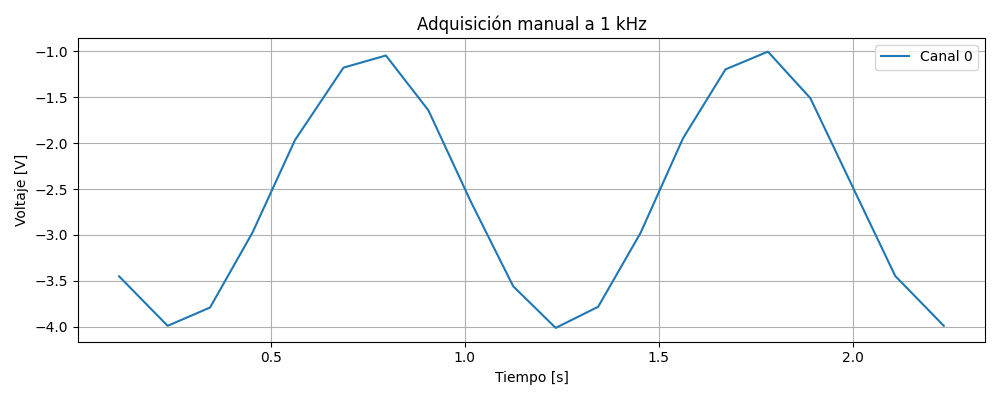
\includegraphics[width=0.5678\linewidth]{Figures/02_06_2025/Ploteo_placa_pyIOTech.png}
	
	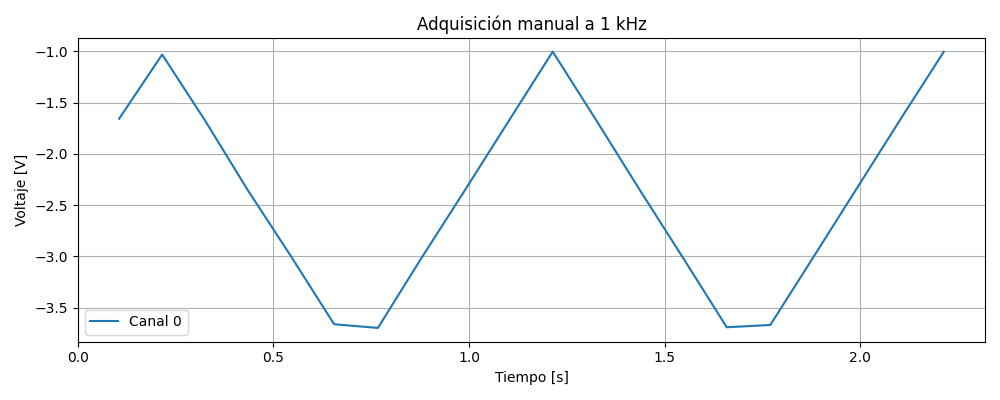
\includegraphics[width=0.5678\linewidth]{Figures/02_06_2025/Ploteo_rampa.png}
	
	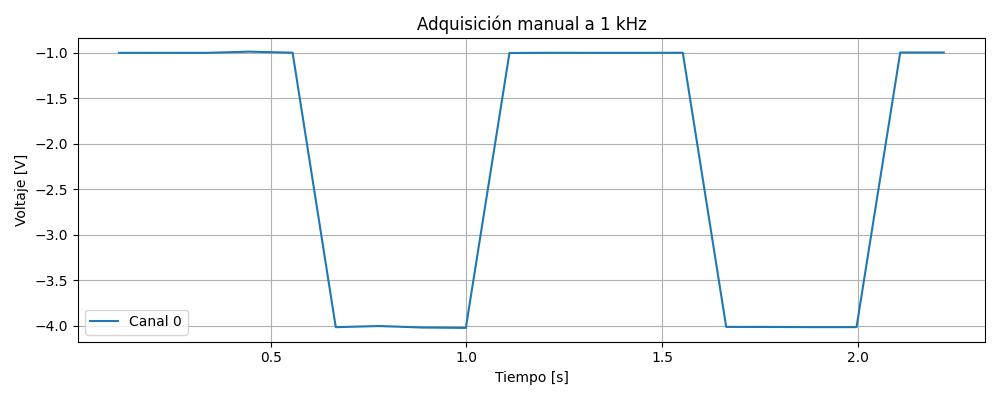
\includegraphics[width=0.5678\linewidth]{Figures/02_06_2025/Ploteo_cuadrada.png}
	\caption{Algunas de las primeras mediciones realizadas con la placa IOTech Personal DAQ 3001 del output del generador Tektronix.}
	\label{fig:ploteoplacapyiotech}
\end{figure}

